%% CHAPTER 13 DIFFERENTIAL EQUATIONS -- dictated by Maximus (26 Oct 2026)
\providecommand{\ddx}{\,\mathrm{d}x}\providecommand{\ddy}{\,\mathrm{d}y}
\newcommand{\DYDX}{\frac{\mathrm{d}y}{\mathrm{d}x}}\newcommand{\DUDX}{\frac{\mathrm{d}u}{\mathrm{d}x}}
\clearpage
\inchap{Differential Equations}
\section{Definition of a Differential Equation}
\begin{theorem}{Differential Equation}
A \textbf{differential equation} is an equation involving a derivative, e.g.\ $\DYDX$, of an unknown function.
\end{theorem}
\section{Solving a Differential Equation}
Solving a differential equation means finding $y$ as a function of $x$ that satisfies the differential equation.
\begin{theorem}{General and Particular Solutions}
\begin{itemize}
\item \textbf{General solution}: a solution containing arbitrary constant(s).
\item \textbf{Particular solution}: a solution where the constant(s) are found from given conditions.
\end{itemize}
\end{theorem}
In this chapter, $C$ and $D$ denote arbitrary constants that are added, and $A$ denotes an arbitrary constant that multiplies.
\subsection{\texorpdfstring{$\DYDX=\mathrm{f}(x)$}{dy/dx = f(x)}}
{\centering{\renewcommand{\arraystretch}{2.2}\begin{tabular}{@{}*{3}{>{$\displaystyle}r<{$}@{}>{$\displaystyle}l<{$}@{\hspace{1.2cm}}}@{}}
\multicolumn{2}{@{}l}{\textbf{Example \stepcounter{exctr}\theexctr}}&\multicolumn{2}{l}{\textbf{Example \stepcounter{exctr}\theexctr}}&\multicolumn{2}{l}{\textbf{Example \stepcounter{exctr}\theexctr}}\\[-2mm]
\DYDX&=3x^{2}&\DYDX&=\mathrm{e}^{2x}&\frac{\mathrm{d}^{2}y}{\mathrm{d}x^{2}}&=6x\\
&\quad\vdots&&\quad\vdots&&\quad\vdots\\
y&=x^{3}+C&y&=\frac12\mathrm{e}^{2x}+C&y&=x^{3}+Cx+D\\
\end{tabular}\par}}
\subsection{Method of Separable Variables}
When a differential equation has ``$y$'' terms, we apply the method of separable variable. Divide the expression in terms of $y$ to the LHS, and keep all $x$ terms on the RHS.
\begin{center}\fbox{\rule[-3mm]{0pt}{10mm}\quad\fhlm{\DYDX=\mathrm{f}(y)\,\mathrm{g}(x)}\quad}\end{center}
{\centering{\renewcommand{\arraystretch}{2.2}\begin{tabular}{@{}*{3}{>{$\displaystyle}r<{$}@{}>{$\displaystyle}l<{$}@{\hspace{1.2cm}}}@{}}
\multicolumn{2}{@{}l}{\textbf{Example \stepcounter{exctr}\theexctr}}&\multicolumn{2}{l}{\textbf{Example \stepcounter{exctr}\theexctr}}&\multicolumn{2}{l}{\textbf{Example \stepcounter{exctr}\theexctr}}\\[-2mm]
\DYDX&=k(30-y)&\DYDX&=ky(1-y)&\DYDX&=xy^{2}+x+y^{2}+1\\
&&&&&=x\left(y^{2}+1\right)+\left(y^{2}+1\right)\\
&&&&&=(x+1)\left(y^{2}+1\right)\\
\frac{1}{30-y}\DYDX&=k&\frac{1}{y(1-y)}\DYDX&=k&\frac{1}{y^{2}+1}\DYDX&=x+1\\
&\quad\vdots&&\quad\vdots&&\quad\vdots\\
\therefore y&=30-A\mathrm{e}^{-kx}&\therefore y&=\frac{1}{1+A\mathrm{e}^{-kx}}&\therefore y&=\tan\left(\frac12x^{2}+x+C\right)\\
\end{tabular}\par}}
\begin{info}[title=Note]
If some values of $x$ and $y$ are given (usually initial values $x=0$, $y=y_{0}$), you should solve for the particular solution.
\end{info}
\begin{info}[title=Note: Sketching graphs of solutions]
\begin{minipage}[c]{0.5\linewidth}
\begin{itemize}
\item \textbf{General solution}: family of curves, i.e.\ many possible different curves.
\item \textbf{Particular solution}: one curve.
\end{itemize}
\end{minipage}\hfill
\begin{minipage}[c]{0.46\linewidth}\centering
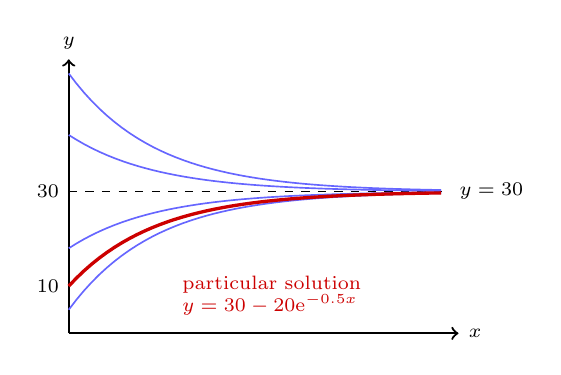
\begin{tikzpicture}[x=0.55cm,y=0.06cm,font=\scriptsize]
\draw[->,thick](0,0)--(9,0) node[right]{$x$};\draw[->,thick](0,0)--(0,58) node[above]{$y$};
\draw[dashed](0,30)--(8.8,30) node[right]{$y=30$};
\foreach \A in {-25,-12,12,25}{\draw[blue!60,semithick,domain=0:8.6,samples=50] plot(\x,{30-\A*exp(-0.5*\x)});}
\draw[red!80!black,very thick,domain=0:8.6,samples=50] plot(\x,{30-20*exp(-0.5*\x)});
\node[left] at (0,10){$10$};\node[left] at (0,30){$30$};
\node[red!80!black,align=left,anchor=west] at (2.4,8){particular solution\\$y=30-20\mathrm{e}^{-0.5x}$};
\end{tikzpicture}\\[-1mm]{\scriptsize Family $y=30-A\mathrm{e}^{-0.5x}$}
\end{minipage}
\end{info}
\begin{info}[title=Note]
Most of the time, graphs of solutions to differential equations in H2 Math have horizontal asymptotes. We can find them by letting $x\to\infty$. Alternatively, let $\DYDX=0$ and solve for $y$ if it is a separable variable differential equation. \fhl{Only if $\DYDX$ is a function of $y$ alone.}
\end{info}
\clearpage
\section{Substitution}
Given a differential equation, it may sometimes be impossible to separate the variables. In such cases, a substitution will be given to you (do not come up with your own).
\exlab
{\small (DHS 2025 Prelim P1 Q1)} It is given that $2xy\DYDX=x^{2}-y^{2}$ where $x>0$, $y<0$. Using the substitution $u=\dfrac{y}{x}$, show that the differential equation can be transformed to $\dfrac{2u}{1-3u^{2}}\DUDX=\dfrac{1}{x}$. Hence find the general solution of $y$ in terms of $x$.\par\medskip
\noindent\textbf{Step 1: Differentiate the substitution}
\cdisp{u=\frac{y}{x}\ \Rightarrow\ y&=ux\\{\color{blue}\DYDX}&{\color{blue}{}=\DUDX x+u}\quad\ldots(1)}
\noindent\textbf{Step 2: Substitute the substitution}
\cdisp{2xy\DYDX&=x^{2}-y^{2}\\2x{\color{red}(ux)}{\color{blue}\left(x\DUDX+u\right)}&=x^{2}-{\color{red}(ux)}^{2}\\&\;\;\vdots\\\frac{2u}{1-3u^{2}}\DUDX&=\frac{1}{x}\quad\text{(shown)}\\&\;\;\vdots\\3u^{2}&=1-\frac{A}{x^{3}}\\\left(\frac{y}{x}\right)^{2}&=\frac13\left(1-\frac{A}{x^{3}}\right)\\\therefore y&=-\sqrt{\frac{x^{2}}{3}\left(1-\frac{A}{x^{3}}\right)}=-x\sqrt{\frac13\left(1-\frac{A}{x^{3}}\right)}\quad(\because y<0)}
\begin{caution}
\textbf{\large VERY IMPORTANT NOTE}\par\smallskip
For substitution in differential equations, always remember to substitute the original variables ($x$ and $y$) back into the equation!
\end{caution}
\begin{caution}
\textbf{\large SUPER ULTRA IMPORTANT NOTE}\par\smallskip
The variable in the substitution is \textbf{NOT A CONSTANT} unless otherwise stated!\par\smallskip
Example: $y=ux^{2}$ (product rule: $u$ and $x^{2}$ are both variables)
\cdisp{\textcolor{red}{\text{\ding{55}}}\quad\DYDX=2ux\qquad\qquad\textcolor{green!45!black}{\text{\ding{51}}}\quad\DYDX=x^{2}\DUDX+u(2x)=x^{2}\DUDX+2ux}
\end{caution}
